\documentclass[convert]{standalone}

\usepackage{tikz}
\usepackage{graphicx}
\pagestyle{empty}

% INT_AY22_L28-Fig09_EM_wave.png

\begin{document}
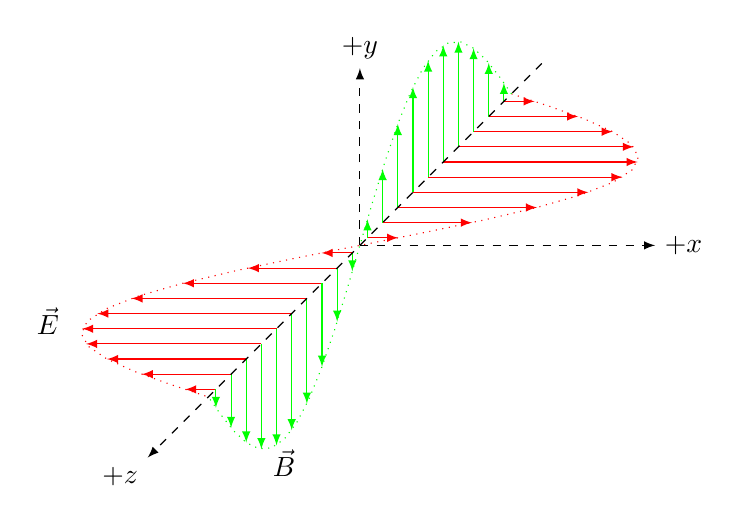
\begin{tikzpicture}[> = latex]

	% Definitions
	
	\def\E{2.5}		% Magnitude of E field
	\def\B{1.5}		% Magnitude of B field
	\def\L{10}		% Wavelength

	% E, B fields

	\foreach \z in {0.25, 0.75, ..., 10}
	{
		\draw [red, ->] (0, 0, \z) -- ({\E * sin(360 * \z / \L)}, 0, \z);
		\draw [green, ->] (0, 0, \z) -- (0, {\B * sin(360 * \z / \L)}, \z);
	}
	
	% Envelopes for fields
	
	\draw [dotted, red] plot [domain = 0:10, variable = \z] ({\E * sin(360 * \z / \L)}, 0, \z);
	\draw [dotted, green] plot [domain = 0:10, variable = \z] (0, {\B * sin(360 * \z / \L)}, \z);
	
	% Line of propagation + axes
	
	\draw [dashed, ->] (0, 0, 0.5 * \L) -- (1.5 * \E, 0, 0.5 * \L) node [right] {$+x$};
	\draw [dashed, ->] (0, 0, 0.5 * \L) -- (0, 1.5 * \B, 0.5 * \L) node [above] {$+y$};
	\draw [dashed, ->] (0, 0, -0.1 * \L) -- (0, 0, 1.2 * \L) node [below left] {$+z$};
	
	% Labels for fields
	
	\node at (-1.2 * \E, 0, 0.75 * \L) {${\vec E}$};
	\node at (0, -1.2 * \B, 0.75 * \L) {${\vec B}$};

\end{tikzpicture}
\end{document}